\documentclass[a4paper,
]{scrreprt}

\usepackage{enseatitlepage}

\usepackage{float}
\usepackage{amsmath}
\usepackage[final]{pdfpages} 

\usepackage{multirow}

% Pour avoir une police sans serif (plus lisible)
\renewcommand{\familydefault}{\sfdefault}

\renewcommand{\labelenumii}{\arabic{enumi}.\arabic{enumii}}

% Title Page
%\titlehead{Document de travail}
\title{Conversion d'Energie I}
%\subtitle{DEP\_1322}
\subject{TD}
\author{Alexis MARTIN}
\date{2023}
%\degree{1\textsuperscript{re} année AB}

\usepackage{lipsum}

\begin{document}
\maketitle

\chapter{Alimentation d’un microprocesseur}

On souhaite alimenter un microprocesseur STM32H4 à l'aide d'une batterie. Le cahier des charges est le suivant :

\begin{itemize}
\item Batterie LiPo 2S $V_{in} = 7.4\ V$
\item Tension d’alimentation du microprocesseur : $V_{out}=3.3\ V$
\item Ondulation de tension max en entrée du microprocesseur : $\Delta V_S = 50\ mV$
\item Courant nominal de sortie : $I_S = 200\ mA$
\item Ondulation de courant : 30\%
\end{itemize}

Pour cela, on souhaite utiliser le composant suivant : \textbf{LT1959} dont un extrait de la documentation est en annexe. On supposera dans cet exercice que les \underline{\textbf{composants sont}} \underline{\textbf{parfaits}}, et que le Buck fonctionne en régime de \underline{\textbf{conduction continue}}.

\begin{enumerate}

\item \textbf{Étude du Buck}

\begin{enumerate}

\item Tracer le circuit permettant d'utiliser ce composant en fonctionnement Buck (la valeur des composants passifs n'est pas demandée). Pour la broche 6 $\overline{SHDN}$, on supposera que le Buck est toujours en fonctionnement.

\begin{center}
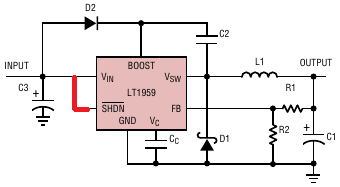
\includegraphics[width=0.8\linewidth]{TD_Buck/Correction/fig/Q1_1.png}
\end{center}

\item On suppose que le processeur absorbe un courant $I_s$ constant égal au courant nominal et que la tension de sortie est constante (on néglige l'ondulation de la tension de sortie). Tracer l'allure de la tension $V_{SW}$ en sortie du composant \textbf{LT1959}, la tension $V_{ce}$ aux bornes du transistor $Q_1$ et le courant $I_{L}$ dans l'inductance de sortie. En déduire la relation entre la tension d'entrée $V_{in}$, $V_{out}$ et le rapport cyclique $\alpha$ du hacheur.

\begin{center}
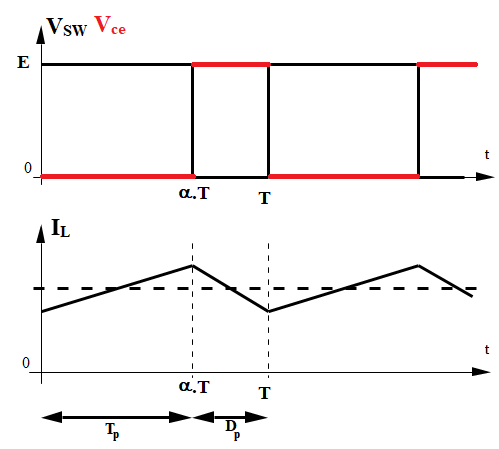
\includegraphics[width=0.7\linewidth]{TD_Buck/Correction/fig/Q1_2.png}

$V_{out}=<V_{SW}>=\alpha V_{in}$
\end{center}

\item Si la tension de sortie est bien régulée, quelle sera la valeur du rapport cyclique $\alpha_n$ imposé par le \textbf{LT1959} ?

\begin{center}
$\alpha=\dfrac{V_{out}}{V_{in}}=\dfrac{3.3}{7.4}\approx0.45$
\end{center}

\item Justifier que ce composant est adapté au cahier des charges. Peut-on utiliser une batterie LiPo 1S ($3.7 V$) à la place de la LiPo 2S ?

\begin{center}
Tension d'entrée min : 4 V $\rightarrow V_{in}>4\ V$

Tension de sortie min : 1.21 V $\rightarrow V_{out}>1.21\ V$

Courant de commutation max : 4.5 A $\rightarrow$ Courant à commuter : $I_S+\Delta I_s/2 =0.2+0.2*0.15=0.23<4.5\ A$

LiPo 1S : $3.7\ V < 4\ V\ \rightarrow$ ne peut pas fonctionner directement avec ce composant
\end{center}

\item A partir de la documentation, quelle est la fréquence de découpage du hacheur ?

\begin{center}
$f_{SW}=500\ kHz$
\end{center}

\item Calculer l'ondulation de courant $\Delta I_{L}$ dans l'inductance de sortie, en fonction de l'inductance $L_1$ placée. En déduire la valeur de l'inductance afin de respecter le cahier des charges.

\begin{center}
Entre 0 et $\alpha T$ : $V_L=V_{in}-V_{out}=L\dfrac{dI_L}{dt} \rightarrow \Delta I_L=(V_{in}-V{out}).\dfrac{\alpha T}{L}$

$\Delta I_L=\dfrac{\alpha .(1-\alpha).V_{in}.T}{L}$

$L>61\mu H$
\end{center}

\item Tracer la tension de sortie en tenant compte de l'ondulation de tension. Calculer la valeur du condensateur de sortie $C_1$ à choisir afin de respecter le cahier des charges.

\begin{center}
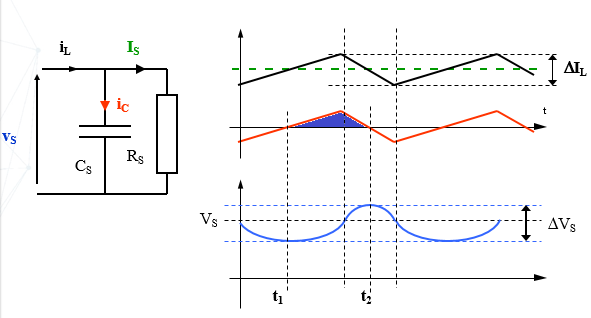
\includegraphics[width=0.7\linewidth]{TD_Buck/Correction/fig/Q1_7.png}

$$t_1=\dfrac{\alpha.T}{2}\ \ \ \ \  t_2=\dfrac{(1+\alpha).T}{2}$$

$$\Delta V_C=\dfrac{1}{C_1}\int_{t_1}^{t_2}i_C(t).dt=\dfrac{1}{C_1}.\dfrac{1}{2}.\dfrac{\Delta I_S}{2}.(t_2-t_1)$$

$$\rightarrow C_S=\dfrac{\alpha.(1-\alpha).V_{in}}{8.f_{SW}^2.L.\Delta V_S}=300\ nF$$
\end{center}

\item Que se passe-t-il si le microprocesseur consomme peu de courant (mode veille par exemple) ?

\begin{center}
Conduction discontinue $\rightarrow$ si $\alpha$ est fixe, $V_S$ augmente (potentiellement jusqu'à $V_{in}=7.4\ V$ si le processeur ne consomme aucun courant)
\end{center}

\end{enumerate}

\item \textbf{Etude de la commande}

Dans cette partie, on s'intéresse à la commande du Buck. Pour cela, on utilise le schéma simplifié suivant :

\begin{figure}[h]
\centering
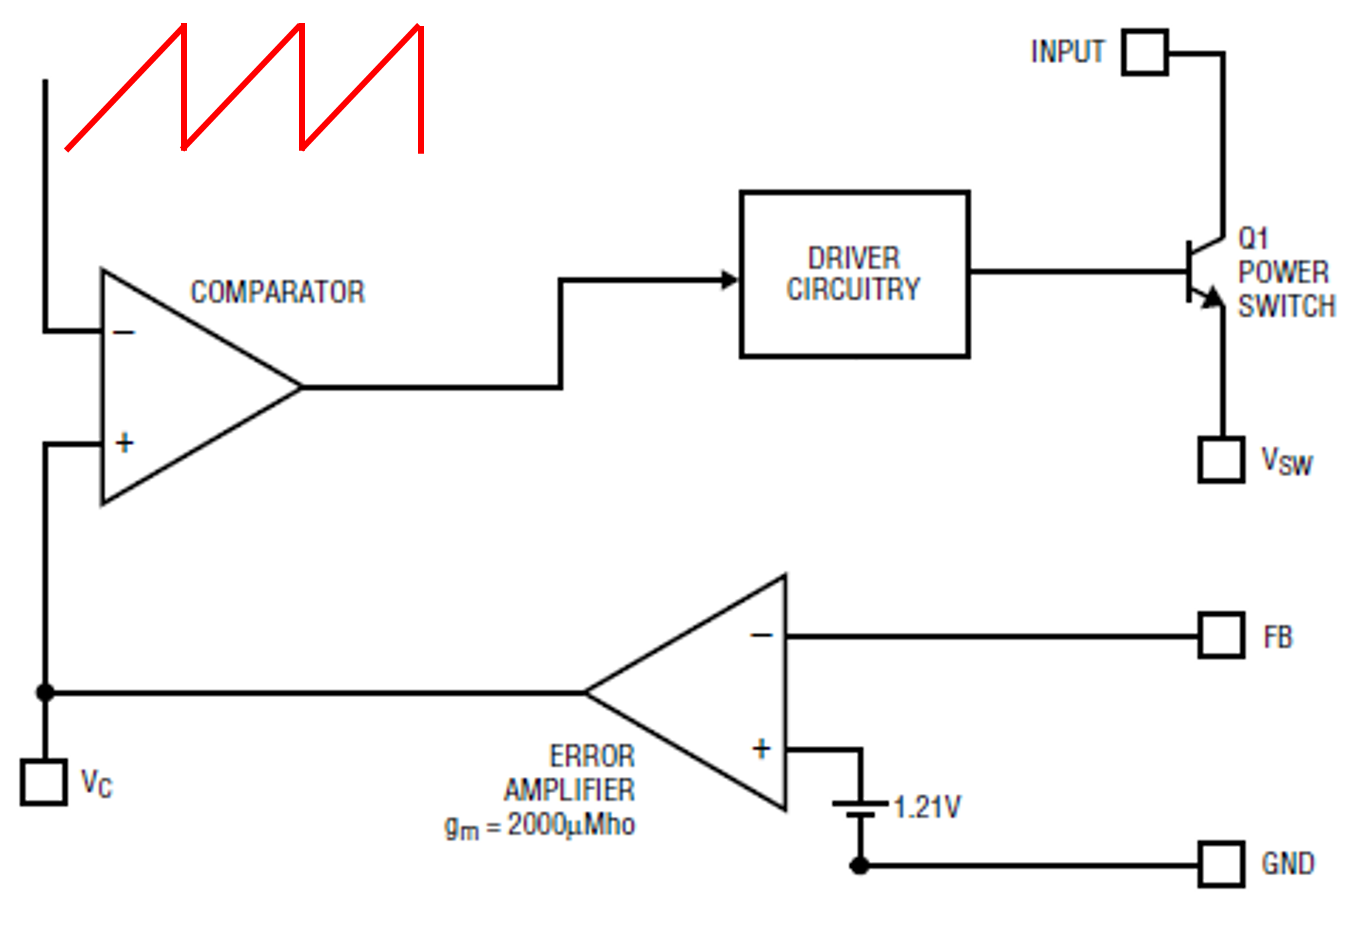
\includegraphics[width=0.8\linewidth]{TD_Buck/fig/Buck_regul.png}
\caption{Simplified internal control}
\end{figure}

Le signal en dent de scie évolue entre 0 et 2 V, avec une fréquence égale à la fréquence de découpage du hacheur. 

\begin{enumerate}

\item Choisir les valeurs des résistances à connecter sur la broche \textit{FB} afin d'avoir la tension de sortie demandée. On utilisera pour cela les valeurs de résistances de la série E12.

(Valeurs de la série E12 : 100, 120, 150, 180, 220, 270, 330, 390, 470, 560, 680, 820).

\begin{center}
Pont diviseur de tension : $\dfrac{R_2}{R_1+R_2}=\dfrac{1.21}{3.3}\rightarrow R_1\approx 1.73.R_2$
$$R_1=470\ k\Omega\ \ \ \ \ \ \ R_2=270\ k\Omega$$
\end{center}


\item Pour une tension $V^+=0.5 V$ à l'entrée du comparateur, tracer le signal en sortie du comparateur. En déduire l'expression qui lie la tension $V^+$ du comparateur et la valeur du rapport cyclique $\alpha$ du hacheur.

\begin{center}
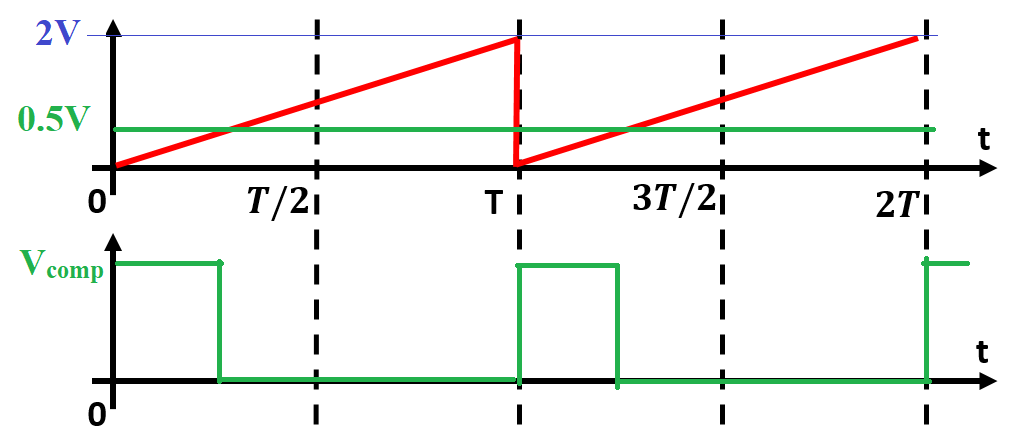
\includegraphics[width=0.7\linewidth]{TD_Buck/Correction/fig/Q2_1.png}
$$V^+=2.\alpha$$

\end{center}

On modélise le convertisseur asservi avec le schéma bloc suivant :

\begin{figure}[H]
\centering
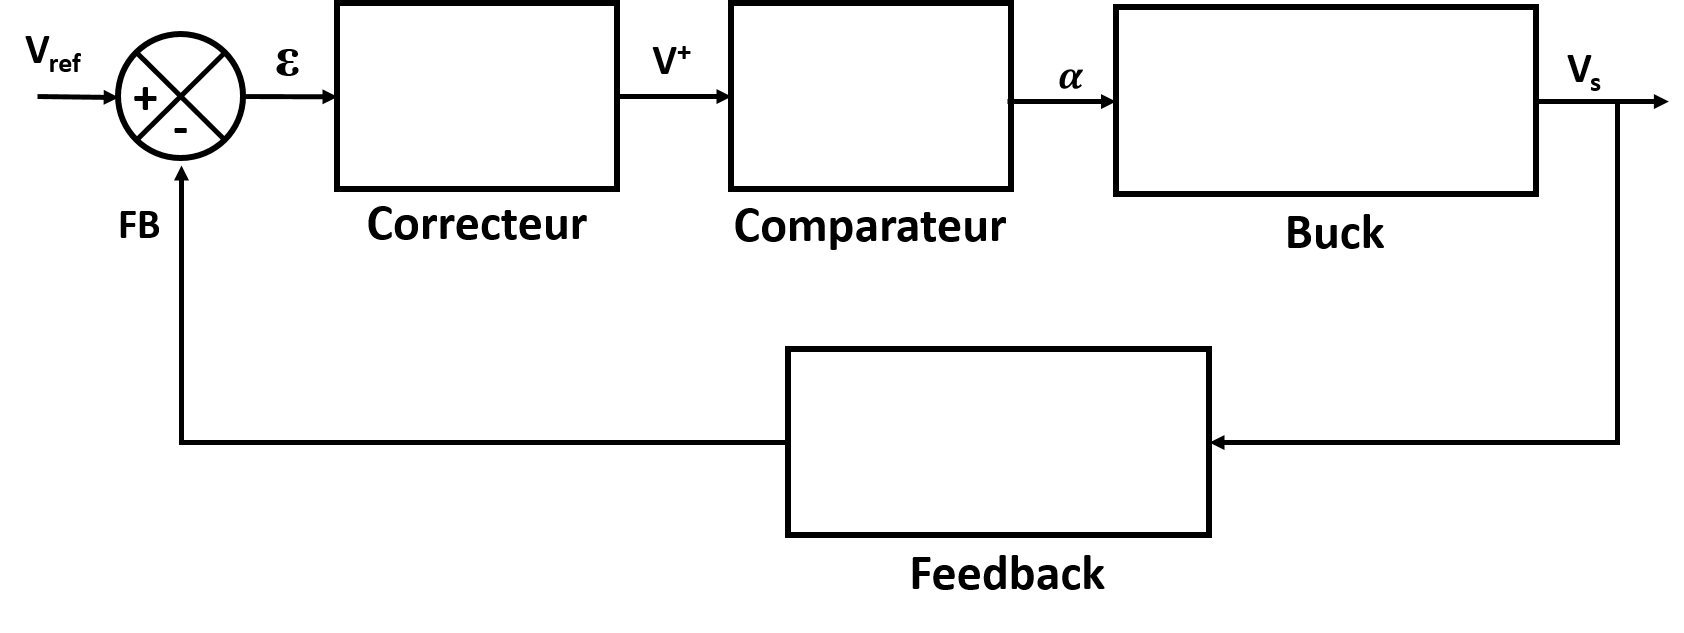
\includegraphics[width=0.8\linewidth]{TD_Buck/fig/Buck_regul_1.png}
\caption{Global bloc diagramm}
\end{figure}

\item Compléter le bloc ``\textit{Comparateur}''. A l'aide de la partie 1, compléter le bloc ``\textit{Feedback}''

Le bloc ``\textit{Buck}'' est modélisé par un gain statique $K$ correspondant à $\dfrac{V_{s\ moy}}{\alpha}$ et une fonction de transfert correspondant au filtre de sortie de Buck. La résistance $R_m$ symbolise l'impédance d'entrée du microcontrôleur.

\begin{figure}[h]
\centering
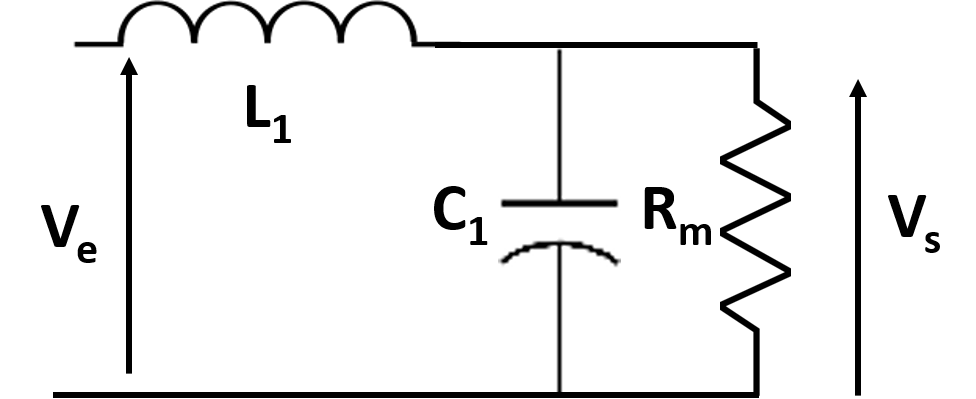
\includegraphics[width=0.65\linewidth]{TD_Buck/fig/Buck_filtre.png}
\caption{Equivalent schematic of the Buck}
\end{figure}

\item Rappeler les valeurs de $L$ et $C$ déterminées à la partie. Déterminer la valeur de $R_m$ lorsque le microcontrôleur absorbe le courant nominal.

\begin{center}

$L=61\ \mu H\ \ \ \ \ \ C=300\ nF$

$R_m=\dfrac{V_{out}}{I_S}=16.5\ \Omega$
\end{center}

\item Déterminer la fonction de transfert correspondant au bloc ``\textit{Buck}''.

\begin{center}
$\dfrac{V_s}{V_e}=\dfrac{1}{1+j.\frac{L_1}{R_m}.\omega-L_1.C_1.\omega^2}$

Fonction de transfert du Buck : $\dfrac{V_s}{\alpha}=\dfrac{V_{in}}{1+j.\frac{L_1}{R_m}.\omega-L_1.C_1.\omega^2}$
\end{center}

\item On place sur la broche $V_c$ un circuit $RC$ série. On suppose que le courant en entrée du comparateur est nul (haute impédance d'entrée). Le bloc ``\textit{Correcteur}'' est donc un proportionnel intégral de la forme $C(p) = K_p(1+\dfrac{1}{T_i.p})$. Déterminer les valeurs de $K_p$ et $T_i$ en fonction de $R$, $C$ et $g_m$.

\begin{center}
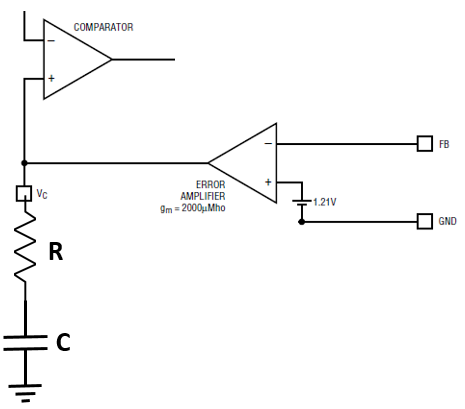
\includegraphics[width=0.55\linewidth]{TD_Buck/Correction/fig/Q2_6.png}
$V^+(j\omega)=(R+\dfrac{1}{j.C.\omega}).I(j\omega)=(R+\dfrac{1}{j.C.\omega}).g_m.\epsilon(j\omega)$

$\dfrac{V^+}{\epsilon}=(R+\dfrac{1}{j.C.\omega}).g_m=R.g_m.(1+\frac{1}{j.R.C.\omega})$

$K_p=R.g_m\ \ \ \ \ \ \ \ \ \ \ \ T_i=R.C$
\end{center}

\item Calculer $R$ afin que le rapport cyclique au démarrage soit environ égal à $\dfrac{\alpha_n}{2}$ et $C$ pour avoir une constante de temps du correcteur 10 fois supérieure à la constante de temps du système non corrigé.

\begin{center}
Au démarrage : $V_{FB}=0$ et le condensateur est déchargé : $V^+=R.g_m.\epsilon=1.2R.g_m$

$\alpha=0.5*1.2R.g_m\rightarrow R=\dfrac{\alpha}{0.6g_m}=186\Omega$

Constante de temps du correcteur : $T_i=R.C>10\sqrt{L_1.C_1}\rightarrow C>\dfrac{10}{R}.\sqrt{L_1.C_1}=230\ nF$
\end{center}

\item En régime établi, déterminer le courant de sortie de l'ampli d'erreur et les tensions aux bornes de $R$, $C$ et $V_c$. En déduire le rapport cyclique et comparer au résultat du 1.3.

Quand t$->$ $\infty$, $\epsilon -> 0$ (thérome de la valeure finale) donc le courant de sortie de l'ampli est nul. 

On a donc $V_{FB}=1.21\ V$ soit $V_{out}=3.3\ V$ comme désiré.

De même, théorme de la valeure finale, $\alpha$ tend vers $\dfrac{R_1+R_2}{R_2}.\dfrac{V_{ref}}{V_{in}}=0.44$


\end{enumerate}

\end{enumerate}

\newpage
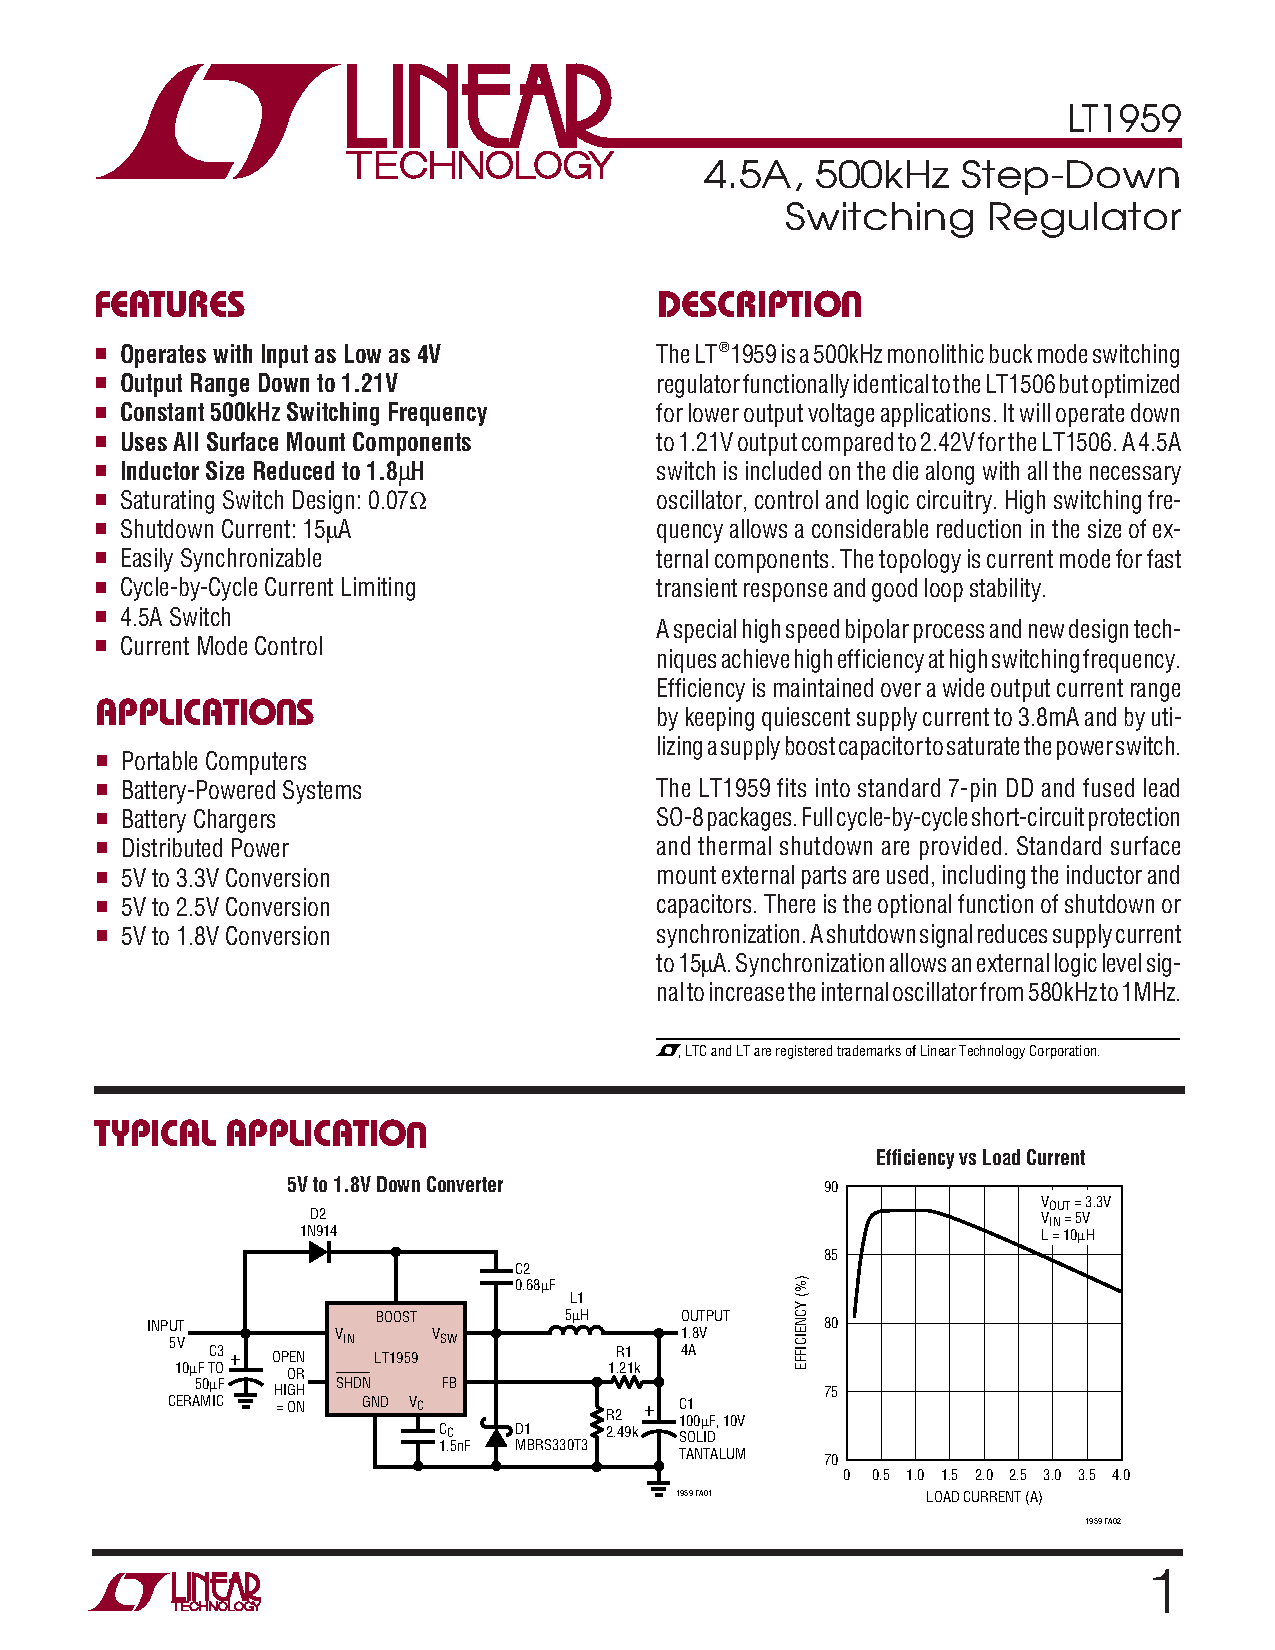
\includepdf[pages=1-4]{TD_Buck/fig/LT1959.pdf}
\includepdf[pages=6-7]{TD_Buck/fig/LT1959.pdf}

%\chapter{4-quadrant chopper used in railway traction}
% Sources: https://www.techniques-ingenieur.fr/base-documentaire/ingenierie-des-transports-th14/materiel-roulant-ferroviaire-42630210/tramways-c4442/performances-en-traction-et-en-freinage-c4442niv10003.html

\textit{The reversible structure of this type of chopper allows for its use in controlling direct current machines in traction, where reversibility is most interesting to exploit. It is used for all power ranges, with the example given here being that of a tramway.}

The tramway is modeled by a "car" powered by a DC machine, itself controlled by a reversible chopper powered by a perfect reversible DC source (catenary type). The simplified diagram of the device is shown in the following figure and corresponds to the described quantities.

\begin{figure}[H]
\centering
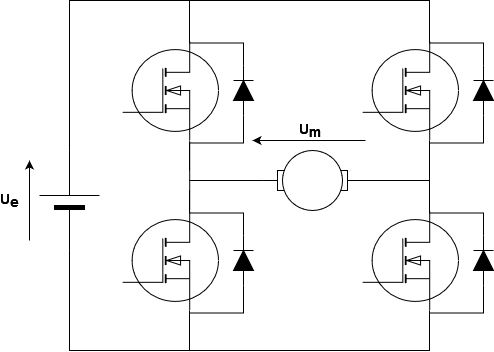
\includegraphics[width=0.55\linewidth]{TD_H4Q/fig/H4Q.png}
\caption{4 Quadrant chopper}
\end{figure}

The chopper is powered by a constant voltage source with a value of $U_E = 1500 V$. It consists of two independent bridge arms controlled at a fixed frequency of $F_d = 2 kHz$. The duty cycles are denoted as follows: $\alpha_1$ for $T_{11}$ and $\alpha_2$ for $T_{21}$, with the control of each arm being complementary. We assume perfect components, diodes, and transistors. Between the two bridge arms, the following control relationship is maintained: $\alpha_1 + \alpha_2 = 1$.

The direct current motor is conventionally modeled by its electromotive force (EMF) $E$, its armature resistance $R$, and its armature inductance $L$; its excitation is kept constant by another device not studied here. The torque constant (equal to the EMF constant) is denoted as $k_\varphi$, and the numerical values are as follows:

$R = 0.2 \Omega$; $L = 25 mH$; $k_\varphi = 7.64 Nm/A$; nominal speed $N_n = 1500 rpm$.

The tramway car constitutes the mechanical load and presents, with respect to the motor shaft, a moment of inertia $J = 200 kg.m^2$. Depending on the trajectory, it also "returns" to this motor shaft a resisting torque denoted as $C_v$.

\begin{enumerate}
\item \textbf{Total complementary control}

\begin{enumerate}
\item Quickly represent the shape of the motor voltage $u_m(t)$ for any duty cycle $\alpha_1$, first less than $0.5$ and then greater than $0.5$.
\item Calculate the average value of this voltage, denoted as $U_m$, as a function of $\alpha_1$.
\end{enumerate}

\item \textbf{Functional description}

In this part, we neglect the current ripple in the motor. In addition, a very fast current control compared to the mechanical time constants allows us to impose the desired value on the motor armature current, denoted as $I_M$, which is constant.

\begin{enumerate}
\item Express the average values (at the switching frequency $F_d$) of the voltage across the motor armature, denoted as $U_M$, and the current drawn by the chopper from the source, denoted as $I_E$, as functions of $\alpha_1$, $U_E$, and $I_M$.
\item The tramway stops on an \textbf{uphill} slope. The weight of the car then exerts a torque on the motor shaft with a value of $C_v = 382 Nm$. What is the duty cycle $\alpha_{10}$ required to keep the tramway at a standstill? What is the current $I_{E0}$ drawn from the power supply (still in average value)?
\item The tramway starts on a level track (neglecting the resisting torque) with a constant acceleration of $5 rad/s^2$ until it reaches the nominal motor speed.

\begin{enumerate}
\item What is the current $I_m$ in the motor?
\item Plot the variation of the duty cycle $\alpha_{1}$ during this acceleration phase.
\item Plot the variation of the current $I_E$ drawn from the power supply during this acceleration phase.
\item Calculate the acceleration time $\Delta t_a$.
\end{enumerate}

\item The tramway travels on a \textbf{downhill} trajectory at a constant speed, with the motor running at its nominal speed. The weight exerts a torque $C_v = 382 Nm$. What is the current $I_{Ed}$ drawn from the power supply? What is the value of the duty cycle $\alpha_{1d}$ that allows for this constant speed operation?
\item Emergency braking downhill: during the previous operation (1.3), the driver requests emergency braking characterized by controlling the armature current to the maximum value tolerable by the chopper and the machine, $I_{max} = 250 A$. We assume that this current is imposed quasi-instantaneously and remains present during the deceleration phase, with the torque related to the weight of the car remaining unchanged at $382 Nm$.

\begin{enumerate}
\item Calculate and represent the time evolution of the motor speed $\Omega(t)$, which represents the tramway speed.
\item Calculate the deceleration time until stop, denoted as $\Delta t_a$.
\item Determine the evolution of the duty cycle $\alpha_1(t)$ during this phase, specifying its value at the beginning of braking and just before the vehicle comes to a stop.
\item Calculate the total energy $E_C$ returned to the source during this braking operation.
\end{enumerate}

\item Represent the operating quadrants of the chopper used during the different phases of the tramway operation.
\end{enumerate}

% \newpage
% \item \textbf{Shifted complementary control of the chopper}

% Here, we propose to change the control of the switches. It is performed according to the diagram shown in the following figure. For each "bridge arm", the control is still complementary with a frequency of $F_d$ (assuming instantaneous switching). To achieve the modulation of the duty cycle, a comparison is made between a modulator ($M_1$ or $M_2$) and the voltage representing the duty cycle $\alpha$, denoted as $v_{alpha}$. We assume that the output of these comparators is a binary signal used to control the switches.

% \begin{figure}[H]
% \centering
% 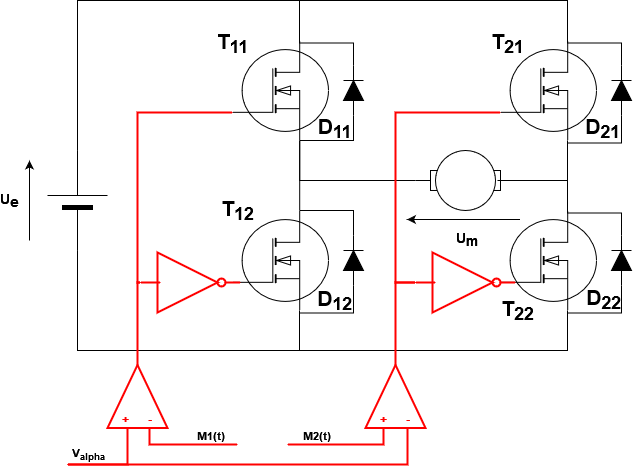
\includegraphics[width=0.6\linewidth]{TD_H4Q/fig/H4Q_decale.png}
% \caption{Shifted control of a 4 quadrant chopper}
% \end{figure}

% The two modulators are shown in the following figure: they are triangular signals in phase opposition with an amplitude of $1 V$. The signal $v_{alpha}$ itself has a maximum amplitude of $1 V$, with its actual amplitude being proportional to the duty cycle $\alpha$.

% \begin{enumerate}
% \item For $\alpha = 0.8$, represent the switching functions $f_1(t)$ and $f_2(t)$ as well as the motor voltage $u_m(t)$.
% \item What is the frequency of the signal $u_m$? What is its "duty cycle", denoted as $\beta$?
% \item For $\alpha = 0.2$, represent the switching functions $f_1(t)$ and $f_2(t)$ as well as the motor voltage $u_m(t)$.
% \item When $\alpha$ is between 0.5 and 1, neglecting the resistance $R$, determine the ripple $\Delta I_M$ in the motor current. What is its maximum value $\Delta I_{M max}$?
% \item What is the advantage of this control compared to total complementary control?
% \end{enumerate}


% \newpage
% \begin{figure}[H]
% \centering
% 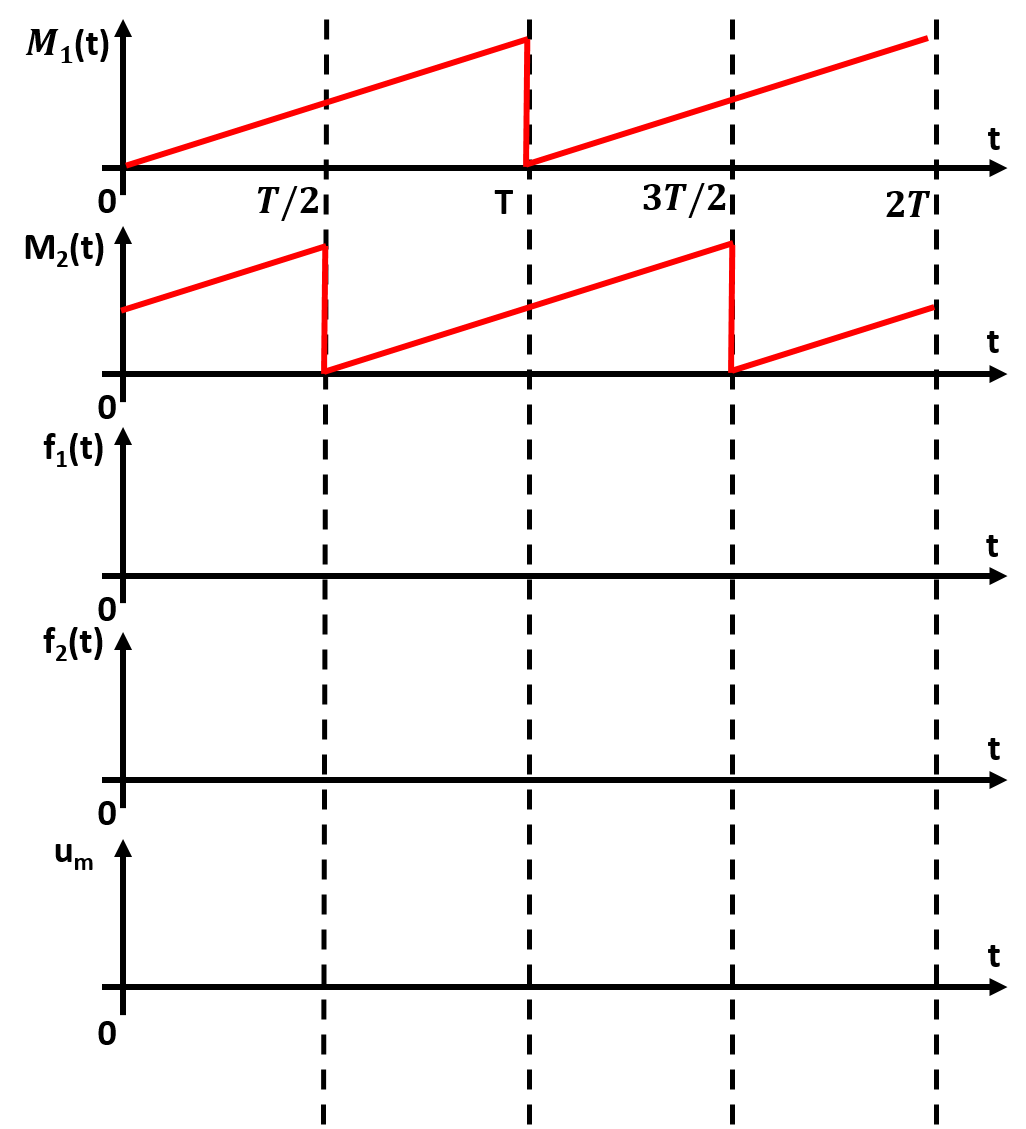
\includegraphics[width=\linewidth]{TD_H4Q/fig/answer.png}
% \caption{Shifted control of a 4 quadrant chopper}
% \end{figure}

%\newpage
%\item \textbf{Independent control}
%
%Here, we propose to change the control of the switches. Transistors $T_{11}$ and $T_{12}$ are still controlled in a complementary manner with the same signal as before. However, transistors $T_{21}$ and $T_{22}$ are now controlled based on the desired output voltage sign: for a positive voltage $U_m$, $T_{22}$ is closed and $T_{21}$ is open, and for a negative voltage $U_m$, $T_{22}$ is open and $T_{21}$ is closed.
%
%\begin{figure}[H]
%\centering
%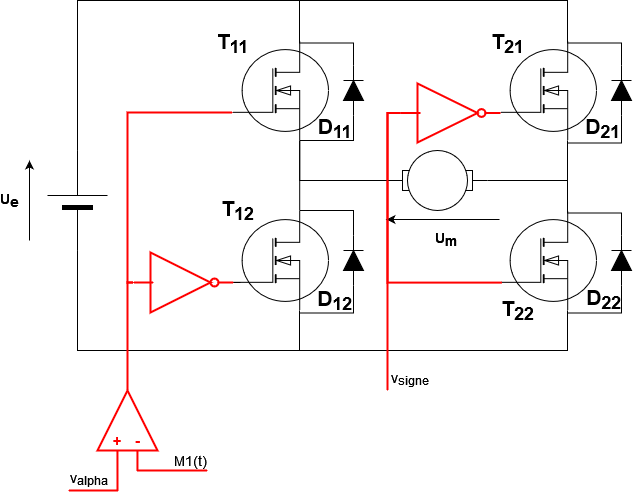
\includegraphics[width=0.6\linewidth]{TD_H4Q/fig/H4Q_indep.png}
%\caption{Independant control 4 quadrant chopper}
%\end{figure}
%
%\begin{enumerate}
%\item Represent the shape of $u_m(t)$ for $\alpha=0.25$ and $v_{signe}=1$
%
%\item Deduce the relationship between the average value of $u_m(t)$ and $\alpha$ when $v_{signe}=1$
%
%\item Represent the shape of $u_m(t)$ for $\alpha=0.25$ and $v_{signe}=0$
%
%\item Deduce the relationship between the average value of $u_m(t)$ and $\alpha$ when $v_{signe}=0$
%
%\item Conclude on the advantages and disadvantages of the different controls
%\end{enumerate}
%
%\begin{figure}[H]
%\centering
%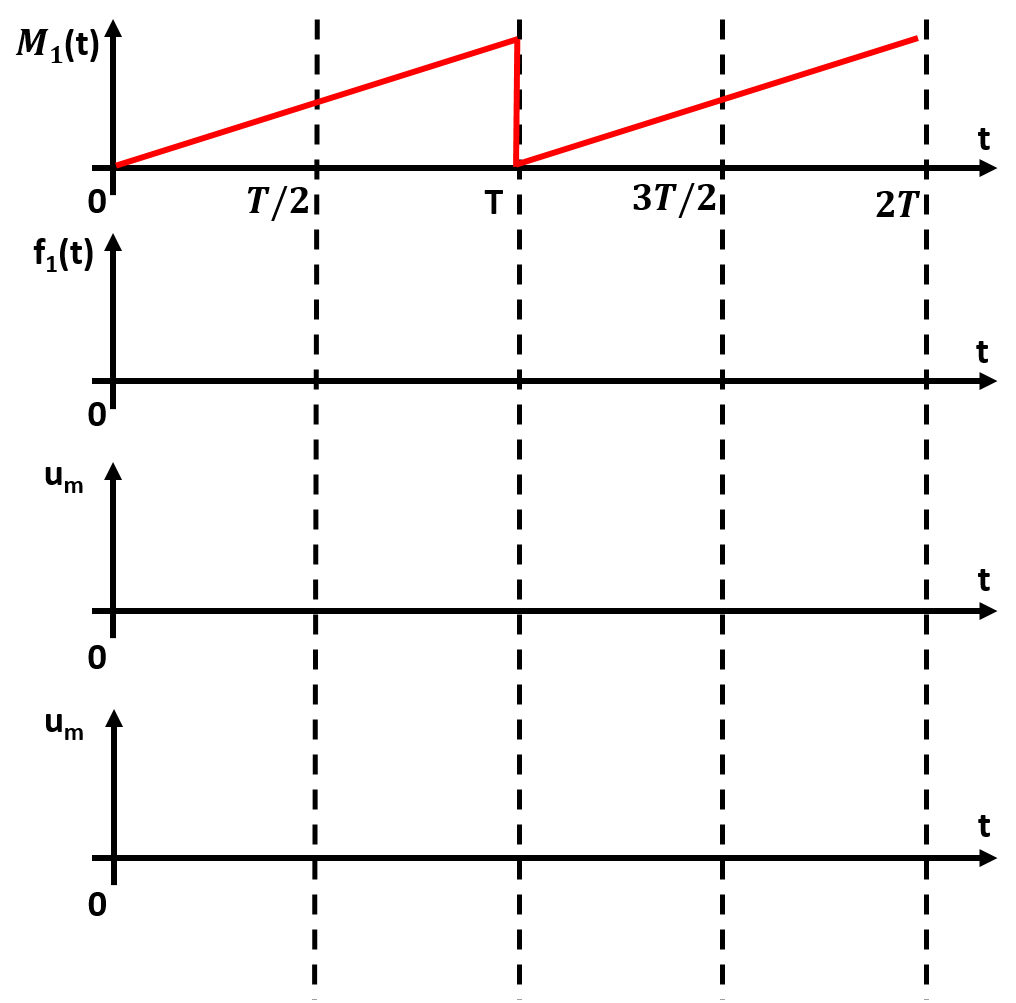
\includegraphics[width=\linewidth]{TD_H4Q/fig/answer2.png}
%%\caption{Shifted control of a 4 quadrant chopper}
%\end{figure}


\end{enumerate}


%\include{TD_Onduleur/TD_Onduleur}

%\chapter{Flyback Switching Power Supply for Battery Charger}
The goal is to use the circuit shown in the following figure to create a 24V battery charger.

\begin{figure}[h]
\centering
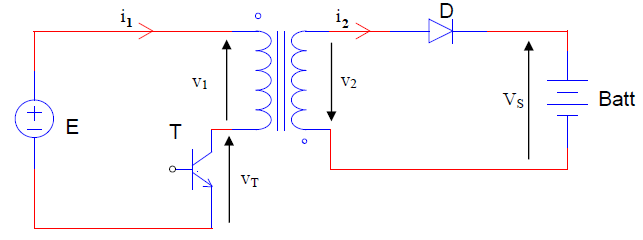
\includegraphics[width=0.9\linewidth]{TD_Flyback/fig/FlybackBatterie.png}
\end{figure}

Let $n_1$ and $n_2$ be the respective numbers of turns in the primary and secondary windings, with the transformation ratio denoted as $m$. The primary magnetizing inductance is denoted as $L_1$, the switching frequency as $f$, and the duty cycle as $\alpha$.

The initially discharged battery has a voltage of $V_{S0} = 20V$ across its terminals. The charging process will be stopped when the voltage across the terminals reaches $V_{S1} = 26V$. However, throughout the analysis, this battery voltage, denoted as $V_S$, will be assumed to be constant on the timescale of the switching.

At the beginning of the battery charging process, it is assumed that the power supply operates in critical mode with a duty cycle of $\alpha_0$, and the average current in the battery is $I_{S0}$.

\vspace{0.25cm}
Numerical values: $E = 300V$; $f = 20 kHz$; $\alpha_0 = 0.5$; $I_{S0} = 10 A$.

\begin{enumerate}

\item \textbf{Start of charging}
\begin{enumerate}
\item Provide the expression of Hopkinson's theorem relating $n_1$, $i_1$, $n_2$, $i_2$, and $R$ (reluctance of the ferrite core, inverse of the specific inductance $A_L$), and $\varphi$ (elementary flux in the core).
\item Plot the waveforms of $i_1$, $i_2$, $\varphi$, $v_T$, and $v_1$ over one switching period.
\item Deduce the expression of the output voltage $V_S$ in terms of $E$, $m$, and $\alpha_0$. Calculate the numerical value of $m$.
\item Determine the expression of the average output current $I_{S0}$ in terms of $L_1$, $\alpha_0$, $m$, $E$, and $f$. Calculate the numerical value of $L_1$.
\item Calculate the energy $W_D$ delivered to the battery per switching cycle using two different methods.
\item Calculate the numerical value of this energy $W_D$ and determine the charging time at constant current for a battery with a "capacity" of 25 Ah.
\end{enumerate}
\item \textbf{End of charging}

During the charging process, the output voltage slowly increases from $V_{S0}$ to $V_{S1}$ while maintaining the duty cycle at $\alpha_0$.
\begin{enumerate}
\item How has the conduction mode of the power supply been modified?
\item Plot the waveforms of $i_1$, $i_2$, $v_T$, and $v_1$ over one switching period.
\item What is the conduction time of the diode D?
\item What is the energy transferred per cycle now? Determine the average current $I_S$ supplied to the battery.
\item What value $\alpha_1$ should be given to the duty cycle to subsequently provide an average charging current of $I_{S1} = I_{S0}/10$?
\end{enumerate}

\item \textbf{Saturation limit}

We are in the critical mode (start of charging).

\begin{enumerate}
\item Determine the expression of the maximum magnetic induction in the ferrite core in terms of $E$, $\alpha$, $T$, $n_1$, and $A_e$ (effective area of the core).
\item Deduce the expression of the minimum value $A_{e\ min}$ of the core area to prevent any saturation of the material. For this purpose, let $B_{sat}$ be the induction value near saturation.
\end{enumerate}

\item \textbf{Winding window area}

We are still in the critical mode (start of charging).

\begin{enumerate}
\item Using the results from the first part, determine the effective value $I_{1\ eff}$ of the current in the transistor in terms of the output current $I_s$, $m$, and $\alpha$.
\item Similarly, express the effective value $I_{2\ eff}$ of the secondary current in terms of $I_s$ and $\alpha$.
\item The chosen current density for both windings made of copper wire is $\delta$. Determine the expression of the total copper area, denoted as $S_{T\ Cu}$, in terms of $I_s$, $\delta$, $n_2$, and $\alpha$. Compare the primary and secondary copper areas.
\item Deduce the minimum winding window area, denoted as $S_B$, if a winding coefficient $k_B$ is chosen ($S_{T\ Cu} = k_B.S_B$).
\end{enumerate}

\item \textbf{Choice of magnetic core}

\begin{enumerate}
\item Based on the results from the previous questions, determine the inequality that the product $A_e.S_B$ of this power supply must satisfy in terms of $B_{sat}$, $P_s$, $T$, $k_B$, $\delta$, and $\alpha$.
\item Calculate the minimum value of this product in $mm^4$ for the following numerical values:

\begin{center}
$P_s = 200 W$; $\alpha = 0.5$; $k_B = 0.5$; $B_{sat} = 0.4 T$; $\delta = 5 A.mm^{-2}$; $f = 20 kHz$.
\end{center}

\item Choose a core from the following list, for which the manufacturer provides the values of $A_e$, $S_B$, and $A_L$ (specific inductance) without air gap, as well as $A_L$ with a 0.5 mm air gap. Note that all these cores are made of the same material, N41.

\vspace{1mm}
\begin{tabular}{| c | c | c | c | c |}
	\hline
	\multirow{2}*{Core} & \multirow{2}*{$A_e\ (mm^2)$} & \multirow{2}*{$S_B \ (mm^2)$} & $A_L$ without air gap & $A_L$ with 0.5 mm air gap\\
	 & & & (nH) & (nH)\\
	\hline
	%RM4 & 11 & 14 & 63 & - - - \\
	\hline
	RM6 & 31 & 32 & 3100 & - - -\\
	\hline
	RM8 & 55 & 57 & 4100 & 160\\
	\hline
	RM10 & 90 & 93 & 5500 & 250\\
	\hline
	RM12 & 125 & 128 & 6000  & 300 \\
	\hline
	RM14 & 170 & 176 & 6800 & 400 \\
	\hline
\end{tabular}

\vspace{1mm}


\item For this choice of core, determine the minimum numbers of turns $n_1$ and $n_2$ to limit the maximum induction in the ferrite core to $B_{sat}$. For these calculations, choose the values of the numbers of turns that are "optimal" for the given numerical values.

\item Will an air gap be necessary to achieve the desired inductance $L_1$?

\end{enumerate}

\begin{figure}[h]
\centering
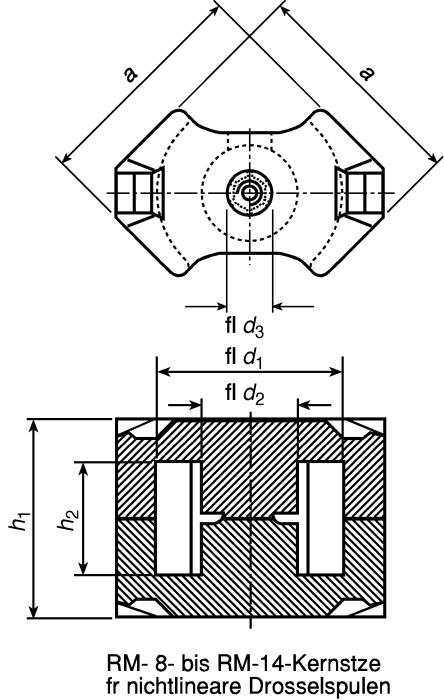
\includegraphics[width=0.5\linewidth]{TD_Flyback/fig/noyau.png}
\end{figure}

\end{enumerate}


%\chapter{Direct Switching Power Supply (Asymmetric FORWARD)}
The purpose of this problem is the simplified study of the switching converter represented in the following figure:

\begin{figure}[h]
\centering
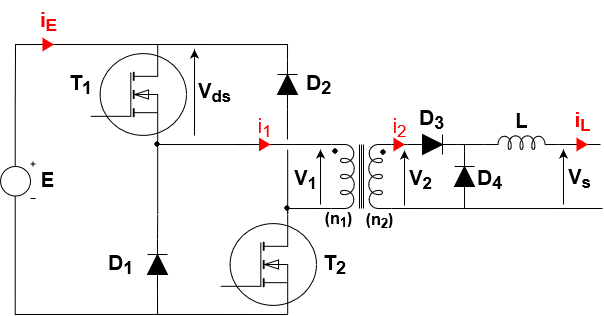
\includegraphics[width=0.85\linewidth]{TD_Forward_Asymetrique/fig/Forward_Asymetrique.png}
\end{figure}

All the semiconductors are assumed to be perfect. The two windings of the transformer are made on the same ferromagnetic core without leakage: all the turns "enclose" the same elementary flux $\varphi$, and the reluctance of this magnetic circuit is denoted by $R$. The output inductance coil $L$ is independent of this transformer. All resistances are neglected.

The control of the transistors is identical, performed at the period $T$, with a duty cycle denoted by $\alpha$: they are therefore conductive
during the interval $[0,\ \alpha.T]$, and blocked during the interval $[\alpha.T,\ T]$.

The output voltage $V_s$ is assumed to be constant throughout the study, and the device will be kept in total demagnetization at each operating cycle. We are only interested in the continuous conduction mode in the output inductance $L$, so its current never becomes zero: $i_L > 0$.

\begin{enumerate}
\item \textbf{General operation of the power supply}

In this part, we will study the operation of the power supply. We will assume that it operates in \textbf{total demagnetization}, meaning that at the end of a period, the magnetic flux in the transformer is zero. We will plot the time curves of $\varphi$ (magnetic flux in the transformer), $v_1$, $v_2$, $v_{DS}$ (drain-source voltage of transistor $T_1$), $v_L$, $i_1$, $i_2$, $i_L$, and $i_E$.

\begin{enumerate}

\item Considering the directions of the windings shown in the diagram and the directions of measurement of the different currents and voltages:
\begin{enumerate}
\item Give the expression of the voltages $v_1$ and $v_2$ as a function of the flux $\varphi$
\item Express the Hopkinson's law relating the currents $i_1$ and $i_2$ to the same flux $\varphi$ using the number of turns and the reluctance $R$.
\end{enumerate}

\item We consider the interval $[0,\ \alpha T]$: we assume that the initial flux at $t = 0$ is zero (total demagnetization)
\begin{enumerate}
\item Determine the voltage $v_1$ applied to the primary winding
\item Deduce the voltage $v_2$ as well as the state of diodes $D3$ and $D4$
\item Give the expression of the voltage $v_L$ across the output inductance in terms of the number of turns, $E$, and $V_S$
\item Express the evolution of the flux $\varphi (t)$ during this time interval
\item Express the current $i_2$ in terms of $i_L$
\item Using the Hopkinson's law and the previous results, determine the expression of the primary current $i_1$ in terms of $i_L$ and the flux $\varphi$ using the number of turns and the reluctance $R$
\item At the instant $\alpha T$, the end of this first time interval, we assume that the flux has become equal to $\varphi_0$. Deduce the expression of this value of $\varphi_0$ in terms of $E$, $n_1$, and $\alpha T$
\end{enumerate}

\item We consider the interval $[\alpha T,\ T]$: all transistors are blocked.
\begin{enumerate}
\item At $t=\alpha T$, determine the state of diodes $D1$ and $D2$. What are the values of voltages $v_1$ and $v_2$? Deduce the state of diodes $D3$ and $D4$
\item Deduce the expression of $v_L$ in terms of $V_S$
\item Express the evolution of the flux $\varphi(t)$ during this time interval
\item At what instant $t_0$ does the flux become zero? Give a condition on $\alpha$ for the system to operate in total demagnetization
\item What happens next until the end of the period T?
\end{enumerate}

\item The power supply is intended to produce a constant voltage of 24 V from the perfectly filtered single-phase rectified network, $E = 300 V$. The transmitted power is $P_n = 600 W$, and the switching frequency is $f = 50 kHz$. We choose to operate the power supply around the nominal duty cycle $\alpha = 0.4$.
\begin{enumerate}
\item Calculate the turns ratio $n_2/n_1$
\item Calculate the average value $I_s$ of the current $i_L$
\item Calculate the minimum value to be given to the inductance $L$ to limit the peak-to-peak ripple of the current $i_L$ to 5\% of its average value $I_s$. \underline{Keep this} \underline{value of $L$ for the following calculations}
\item Deduce the maximum value $I_{1\ max}$ of the current in the transistor when neglecting the magnetizing current
\end{enumerate}

\end{enumerate}

\item \textbf{Transformer dimensioning}

\begin{enumerate}
\item To justify the previous assumption, determine the minimum value of the magnetizing inductance $L_1$ (seen from the primary winding) that makes the maximum no-load current less than $I_{1\ max} /20$

\item \underline{Neglecting the ripple of the current $i_L$ and the magnetizing current}, determine the rms values $I_{1\ eff}$ and
$I_{2\ eff}$ of the currents $i_1$ and $i_2$ in terms of $I_s$, $n_1$, $n_2$, and $\alpha$
\item Determine, with these same assumptions, the minimum winding area $S_B$ required in terms of current density $\delta$, winding coefficient $k_B$, $I_s$, $n_2$, and $\alpha$
\item Also give the expression of the minimum cross-sectional area $A_e$ of the core that avoids core saturation by maintaining a maximum induction below $B_{max}$
\item Deduce the minimal sizing product $A_e.S_B$ of this transformer in terms of the duty cycle, the different characteristic parameters of this power supply, including its output power $P_S$, and its switching frequency $f$

\end{enumerate}

\end{enumerate}

\begin{figure}[h]
\centering
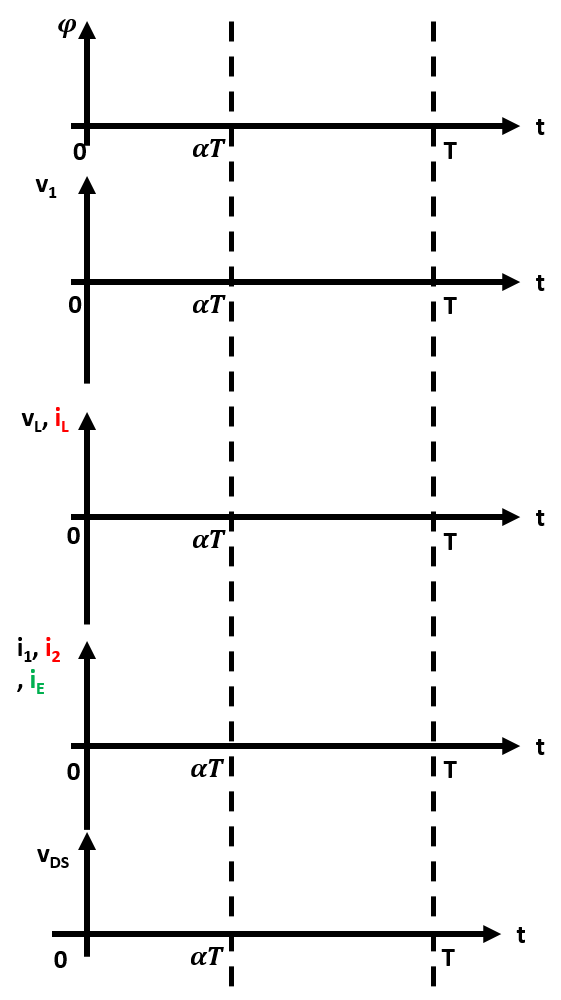
\includegraphics[width=0.85\linewidth]{TD_Forward_Asymetrique/fig/doc_reponse.png}
\end{figure}





\end{document}
